% ==============================
% Chapter 1 – Introduction
% ==============================

\chapter{Introduction}

% --------------------------------
% 1.1 Introduction
% --------------------------------

\section{Introduction}

Access to affordable and trustworthy rental accommodation is a fundamental need for the large population of students and young professionals who migrate to urban centres across Pakistan every year. Cities such as Multan, Lahore, and Islamabad host major universities and employment hubs that attract thousands of individuals who require short-term, low-cost living arrangements close to their place of study or work. For this segment, the ideal accommodation is rarely an entire house; instead it is a single room, a shared room, a bed space, or a hostel seat that fits a limited student or entry-level budget.

The current rental ecosystem, however, is poorly suited to this demand. The process is dominated by informal property dealers and word-of-mouth referrals. Prospective tenants typically rely on local brokers who charge substantial commissions, on unstructured social media groups where listings are unverified, or on classified websites that are designed primarily for full-house and commercial rentals. None of these channels offers a reliable mechanism to confirm that a listed property genuinely exists, that the advertised landlord is the true owner, or that a tenant is who they claim to be.

A second, equally significant problem is the absence of any systematic approach to roommate selection. Because shared accommodation is inherently a social arrangement, an incompatible roommate can transform an affordable living solution into a source of constant stress and conflict. At present, roommate selection is left almost entirely to chance, with users having no structured way to evaluate compatibility in terms of habits, study or work routines, cleanliness, and budget expectations.

These shortcomings result in high financial cost, wasted time, exposure to fraud, and avoidable interpersonal conflict. They also represent a clear gap in the digital marketplace: while ride-hailing, food delivery, and e-commerce have all been transformed by dedicated platforms, the micro-rental and roommate matching domain remains fragmented and underserved.

The proposed system, \textbf{Domavi}, is a web-based platform designed to close this gap. Domavi unifies a dedicated micro-rental marketplace, an intelligent roommate matching engine, a multi-layer trust and verification system, commute-based geospatial search, and end-to-end digital process automation within a single application. By bringing structure, transparency, and data-driven decision support to a previously informal process, Domavi aims to make shared housing safer, cheaper, and significantly easier to navigate for its target users.

% --------------------------------
% 1.2 Vision Statement
% --------------------------------

\section{Vision Statement}

The vision of Domavi is to become the most trusted digital platform for affordable shared accommodation in Pakistan, serving primarily students and young professionals who seek single rooms, bed spaces, and hostel accommodation near their universities and workplaces. The platform seeks to eliminate the dependence on informal brokers and unverified listings by establishing a transparent, verification-driven marketplace where every property and every participant is authenticated.

Beyond simply listing rooms, Domavi aspires to redefine the shared-living experience by intelligently matching individuals with compatible roommates based on lifestyle, preferences, budget, and routine. In doing so, the platform addresses both the economic dimension of housing affordability and the social dimension of living harmony. The long-term vision is a safer, more affordable, and more transparent rental culture in which a student arriving in a new city can secure verified accommodation and a compatible roommate within minutes, entirely online, without paying excessive commissions or risking fraud. The uniqueness of Domavi lies in the combination of micro-rental focus, algorithmic roommate compatibility, and layered trust verification within one ecosystem, a combination that no existing local platform currently offers.

% --------------------------------
% 1.3 Related System Analysis
% --------------------------------

\section{Related System Analysis}

Several existing platforms partially address the housing search problem, but none of them target the specific micro-rental and roommate matching needs of students and young professionals in the Pakistani context. This section critically examines representative systems and contrasts them with the proposed solution.

\textbf{General classified marketplaces} such as OLX and similar local listing websites allow individuals to post rental advertisements. While they offer wide reach, they suffer from major weaknesses. Listings are entirely unverified, which exposes users to fraudulent advertisements and fake landlords. The platforms are general-purpose and are not optimised for single rooms or bed spaces, so users must manually sift through large volumes of irrelevant full-house and commercial listings. There is no roommate matching capability, no ownership verification, and no structured booking or agreement workflow.

\textbf{Dedicated property portals} such as Zameen.com focus on property buying, selling, and full-house renting. They provide professional listings and map views but are oriented toward higher-value transactions and full properties rather than affordable single-room rentals. They do not support roommate matching, lifestyle-based compatibility, or the kind of low-cost, short-term arrangements that students require.

\textbf{International roommate platforms} such as Roomster and SpareRoom demonstrate the value of roommate-oriented features and are useful reference points. However, they are designed for Western markets, often operate behind paywalls, lack localised verification suited to Pakistani identity documents such as the CNIC, and are not commonly used or trusted within the local market. Their compatibility features are also typically limited to basic preference filters rather than a weighted, multi-factor compatibility score.

\textbf{Informal social media groups}, particularly on Facebook and WhatsApp, are widely used in practice. They are free and community-driven but completely unstructured. There is no verification, no search or filtering, no compatibility assessment, and no protection against scams, making them unreliable for serious accommodation decisions.

In contrast, Domavi is purpose-built for the micro-rental segment. It combines verified listings, a multi-layer trust system tailored to local identity documents, a weighted roommate compatibility engine, commute-based proximity search, and an automated booking and agreement workflow. The comparative analysis below summarises the key weaknesses of existing solutions and the corresponding improvements offered by Domavi.

\vspace{0.5cm}

\begin{table}[h!]
\centering
\caption{Comparative Analysis of Existing Systems}
\renewcommand{\arraystretch}{1.3}

\begin{tabularx}{\textwidth}{|p{3cm}|X|X|}
\hline
\textbf{Application Name} & \textbf{Identified Weaknesses} & \textbf{Proposed Improvements in Domavi} \\
\hline
OLX / General Classifieds &
\begin{itemize}[leftmargin=*, noitemsep, topsep=0pt]
    \item Unverified, fraud-prone listings
    \item Not optimised for single rooms
    \item No roommate matching
\end{itemize}
&
\begin{itemize}[leftmargin=*, noitemsep, topsep=0pt]
    \item Multi-layer verification
    \item Dedicated micro-rental marketplace
    \item Algorithmic roommate matching
\end{itemize}
\\
\hline
Zameen.com &
\begin{itemize}[leftmargin=*, noitemsep, topsep=0pt]
    \item Focused on full houses / sales
    \item High-value, not student budget
    \item No compatibility features
\end{itemize}
&
\begin{itemize}[leftmargin=*, noitemsep, topsep=0pt]
    \item Single rooms and bed spaces
    \item Affordable, student-oriented
    \item Lifestyle-based matching
\end{itemize}
\\
\hline
Roomster / SpareRoom &
\begin{itemize}[leftmargin=*, noitemsep, topsep=0pt]
    \item Designed for Western markets
    \item Paywalled features
    \item No local CNIC verification
\end{itemize}
&
\begin{itemize}[leftmargin=*, noitemsep, topsep=0pt]
    \item Localised for Pakistan
    \item Free core functionality
    \item CNIC and ownership verification
\end{itemize}
\\
\hline
Facebook / WhatsApp Groups &
\begin{itemize}[leftmargin=*, noitemsep, topsep=0pt]
    \item Completely unstructured
    \item No verification or filtering
    \item No fraud protection
\end{itemize}
&
\begin{itemize}[leftmargin=*, noitemsep, topsep=0pt]
    \item Structured search and filters
    \item Verified users and listings
    \item Secure, auditable workflow
\end{itemize}
\\
\hline

\end{tabularx}
\end{table}

% --------------------------------
% 1.4 Project Deliverables
% --------------------------------

\section{Project Deliverables}

The project produces a set of tangible software and documentation artifacts that collectively demonstrate a complete, working micro-rental and roommate matching platform. The principal deliverables are described below.

The core deliverable is a fully functional, responsive web application built on the MERN stack, accessible to tenants, landlords, and administrators through role-specific interfaces. Supporting this application is a documented backend REST API that exposes secure endpoints for authentication, property management, search, booking, payments, messaging, roommate matching, and administration. A structured MongoDB database, designed to store users, properties, roommate profiles, bookings, agreements, payments, conversations, messages, documents, and landlord bank accounts, underpins the entire system.

In addition to the running software, the project delivers complete engineering documentation, including this Software Requirements Specification and Software Design Document, covering use case models, functional and non-functional requirements, architectural and database design, and test cases. The deliverables also include the implemented feature modules that give the platform its distinctive value.

\vspace{0.5cm}

\textbf{List of Deliverables:}

\begin{enumerate}
    \item Micro-Rental Marketplace -- listing, searching, and management of single rooms, bed spaces, and hostels with photos, pricing, and amenities.
    \item Roommate Matching Engine -- a weighted compatibility scoring system that ranks potential roommates by lifestyle, preferences, budget, location, and schedule.
    \item Trust and Verification Module -- multi-layer verification including email/phone confirmation, administrator-reviewed CNIC verification, and property ownership validation.
    \item Commute-Based Geospatial Search -- Google Maps integration enabling proximity-based discovery of accommodation near a chosen university or workplace.
    \item Booking, Payment, and Digital Agreement Workflow -- structured booking requests, online payment recording with administrative confirmation, and auto-generated digital rental agreements in PDF form.
    \item Secure Messaging Module -- real-time, in-app conversations between tenants and landlords.
    \item Administrative Dashboard -- user management, verification review, payment oversight, and platform analytics.
    \item Project Documentation -- SRS, SDD, test documentation, and source code repository.
\end{enumerate}

% --------------------------------
% 1.5 System Limitations / Constraints
% --------------------------------

\section{System Limitations / Constraints}

While Domavi delivers a comprehensive solution, its scope is bounded by a number of technical and practical constraints that are important to acknowledge.

\begin{itemize}
    \item \textbf{Online connectivity dependence} -- The platform is a web application and requires a stable internet connection; it does not provide offline functionality.
    \item \textbf{Third-party service reliance} -- Core features such as map-based search, media storage, and email delivery depend on external services (Google Maps API, cloud storage, and SMTP providers); availability and quota limits of these services constrain the system.
    \item \textbf{Manual verification overhead} -- CNIC and ownership verification require administrator review, which introduces a human-in-the-loop step and limits the speed of fully automated onboarding.
    \item \textbf{Geographic focus} -- The initial release targets selected Pakistani cities and university areas rather than nationwide coverage.
    \item \textbf{Payment handling} -- The system records and confirms payments and bank-transfer details rather than executing live transactions through an integrated payment gateway in the initial version.
    \item \textbf{Resource and timeline constraints} -- As an academic Final Year Project developed by a two-member team within a fixed academic timeline, certain advanced features are scoped for future work rather than the initial release.
\end{itemize}

% --------------------------------
% 1.6 Tools and Technologies
% --------------------------------

\section{Tools and Technologies}

The technology choices for Domavi were guided by the need for rapid development, a single-language full-stack workflow, strong support for real-time and geospatial features, and proven scalability. The platform is built on the MERN stack, which allows JavaScript and TypeScript to be used uniformly across the client and server, reducing context-switching and improving maintainability. MongoDB was selected as the database because its flexible document model and native geospatial indexing are well suited to evolving listing schemas and proximity-based search. React with the Vite build tool provides a fast, component-driven frontend, while Node.js and Express.js power a modular REST API. Supporting libraries provide authentication, media storage, mapping, and document generation.

\begin{table}[h!]
\centering
\caption{Tools and Technologies Used in the Project}
\renewcommand{\arraystretch}{1.3}
\begin{tabularx}{\textwidth}{|p{4.2cm}|p{2.8cm}|X|}
\hline
\textbf{Tool / Technology} & \textbf{Category} & \textbf{Purpose} \\
\hline
React + Vite & Frontend & Component-based, responsive user interface and fast development build \\
TypeScript & Frontend / Backend & Static typing for safer, more maintainable code on both ends \\
Tailwind CSS & Frontend & Utility-first styling and consistent, responsive design \\
Zustand & Frontend & Lightweight client-side state management \\
Node.js + Express.js & Backend & REST API and server-side business logic \\
MongoDB + Mongoose & Database & Document data store with schema modelling and geospatial indexing \\
JSON Web Token (JWT) & Security & Stateless authentication and session handling \\
Google Maps API & Integration & Commute-based search, geocoding, and map display \\
Cloud Media Storage & Integration & Storage of property images and verification documents \\
SMTP / Email Service & Integration & Email verification and notifications \\
PDF Generation Library & Backend & Auto-generation of digital rental agreements \\
Git / GitHub & Tooling & Version control and collaboration \\
\hline
\end{tabularx}
\end{table}

% --------------------------------
% 1.7 Relevance to Course Modules
% --------------------------------

\section{Relevance to Course Modules}

The development of Domavi integrates knowledge drawn from across the BS Information Technology curriculum, demonstrating the practical application of theoretical concepts learned throughout the degree program.

\subsection{Programming Fundamentals}

The project applies core programming principles including modular function design, control flow, exception handling, and object-oriented concepts. The codebase is organised into reusable services and controllers on the backend and composable components on the frontend, reflecting sound structuring, encapsulation, and separation of concerns learned in introductory programming courses.

\subsection{Data Structures and Algorithms}

The roommate matching engine is the clearest application of algorithmic knowledge. It computes a weighted compatibility score across multiple categories, sorts candidate profiles by score to return top matches, and caches previously computed scores for efficiency. Searching, filtering, and ranking of large listing sets also rely on appropriate data-structure and algorithmic choices.

\subsection{Database Management Systems}

Database design concepts such as schema modelling, relationships between collections, indexing, and query optimisation are applied throughout. The MongoDB data model defines structured collections for users, properties, bookings, payments, and agreements, with geospatial and compound indexes used to support efficient proximity search and status-based queries.

\subsection{Software Engineering}

The project follows a complete software engineering lifecycle. Requirement engineering, use case modelling, UML diagramming, architectural design, iterative development, and systematic testing are all applied. This very document, comprising the SRS and SDD, is a direct product of software engineering methodology, while version control and modular architecture reflect professional development practice.

\subsection{Other Relevant Courses}

Web technologies underpin the entire client-server implementation, including REST API design and responsive frontend development. Computer networking concepts inform the use of HTTP/HTTPS and secure communication. Human-computer interaction principles guide the user interface and experience design, while information security concepts shape the authentication, role-based access control, and multi-layer verification mechanisms.

% --------------------------------
% 1.8 Project Schedule
% --------------------------------

\section{Project Schedule}

The development of Domavi was planned and tracked using a project schedule that divided the work into sequential and overlapping phases following the Agile, iterative development approach. The project began with requirement gathering and analysis, followed by system design (SRS and SDD) and database design. Backend and frontend development were carried out in parallel, after which the distinctive modules, roommate matching and the maps and verification integration, were implemented. The final phases covered testing and evaluation, followed by review and deployment. Documentation was maintained continuously throughout the project rather than treated as a single end-stage activity. The Gantt chart below summarises the timeline and the duration of each major activity.

\begin{figure}[h]
\centering
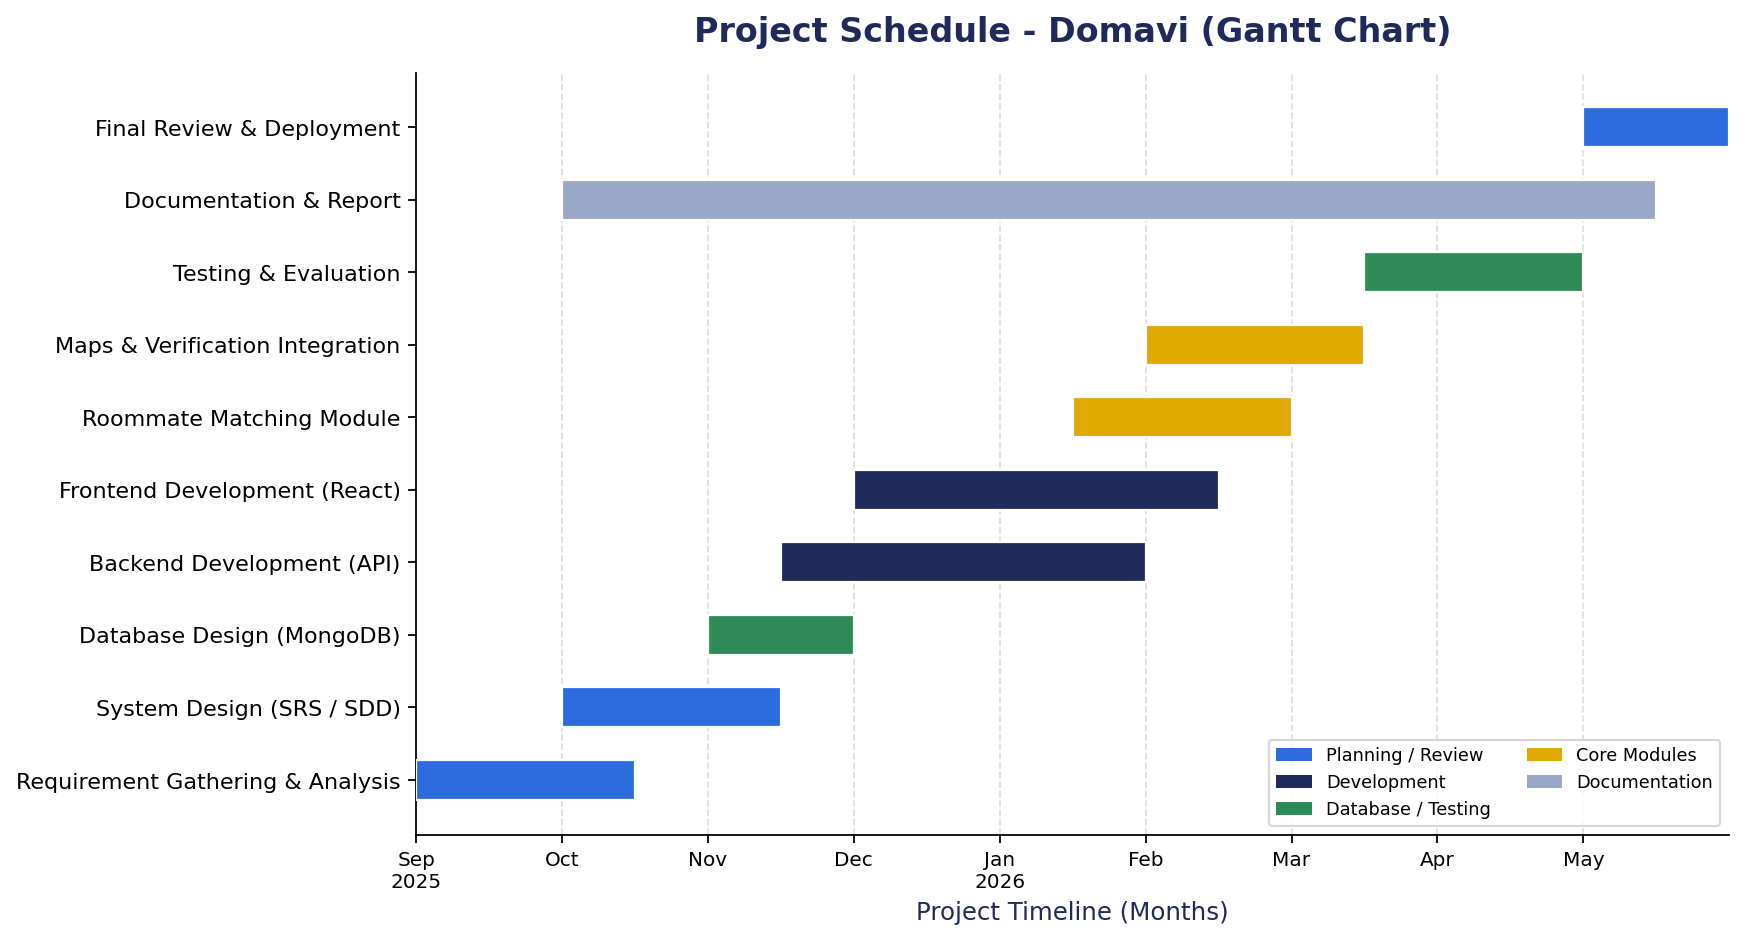
\includegraphics[width=\textwidth]{Figures/Gantt Chart.png}
\caption{Project Schedule (Gantt Chart) of the Domavi Platform}
\label{fig:gantt}
\end{figure}

%%%%%%%%%%%%%%%%%%%%%%%%%%%%%%%%%%%%%%%%%%%%%%%%%%%%%%
\section{Chapter Summary}
%%%%%%%%%%%%%%%%%%%%%%%%%%%%%%%%%%%%%%%%%%%%%%%%%%%%%%

This chapter introduced the background and context of the Domavi platform,
highlighting the high cost, fraud risk, and roommate incompatibility that
characterise the current micro-rental market for students and young
professionals in Pakistan. The vision and strategic objectives of the system
were outlined to establish its intended impact and innovation. A comparative
analysis of related systems identified key limitations in current solutions
such as general classifieds, property portals, international roommate
platforms, and informal social media groups. Project deliverables, system
constraints, selected technologies, and academic relevance were also discussed.

This chapter establishes the foundation for the detailed problem definition
presented in the next chapter.
